%%%%%%%%%%%%%%%%%%%%%%%%%%%%%%%%%%%%%%%%%%%%%%%%%%%%%%%%%%%%%%%%%%%%%%%%%%%%%%%%
%2345678901234567890123456789012345678901234567890123456789012345678901234567890
%        1         2         3         4         5         6         7         8

\documentclass[letterpaper, 10 pt, conference]{ieeeconf}  % Comment this line out if you need a4paper

%\documentclass[a4paper, 10pt, conference]{ieeeconf}      % Use this line for a4 paper

\IEEEoverridecommandlockouts                              % This command is only needed if 
                                                          % you want to use the \thanks command

\overrideIEEEmargins                                      % Needed to meet printer requirements.

% See the \addtolength command later in the file to balance the column lengths
% on the last page of the document

% The following packages can be found on http:\\www.ctan.org
\usepackage{graphicx} % for pdf, bitmapped graphics files
%\usepackage{epsfig} % for postscript graphics files
%\usepackage{mathptmx} % assumes new font selection scheme installed
%\usepackage{times} % assumes new font selection scheme installed
\usepackage{amsmath} % assumes amsmath package installed
\usepackage{amssymb}  % assumes amsmath package installed

\usepackage{subfigure}

\title{Encounter Based Multi Robot Simultaneous Localization and Occupancy Grid Mapping}


% author names and affiliations
% use a multiple column layout for up to three different
% affiliations
\author{RB Choroszucha$^{1}$, C Hyman$^{2}$, and A Collier$^{3}$ % <-this % stops a space
\thanks{$^{1}$ RB Choroszucha is with the School of Naval Architecture and Marine Engineering, University of Michigan.  E-mail: riboch{@}umich.edu}%
\thanks{$^{2}$ C Hyman is with the School of Electrical Engineering and Computer Science, University of Michigan. E-mail: {hymanc}{@}umich.edu}
\thanks{$^{3}$ A Collier is with the School of Electrical Engineering and Computer Science, University of Michigan. E-mail: {amcollie}{@}umich.edu}
}



\begin{document}



\maketitle
\thispagestyle{empty}
\pagestyle{empty}


%%%%%%%%%%%%%%%%%%%%%%%%%%%%%%%%%%%%%%%%%%%%%%%%%%%%%%%%%%%%%%%%%%%%%%%%%%%%%%%%
\begin{abstract}

In this paper we present and implement the algorithm in Howard's 2006 paper: ``Multi-robot simultaneous localization and mapping using particle filters.''  While Howard's method is attractive for its speed, it combines the forward and reverse particle weights, which can result in undesired particle error.  In this paper we propose a modification of the algorithm by using independent particle filters for each robot, and demonstrate that the modified algorithm provides a qualitatively better map, and a more accurate pose estimate.


\end{abstract}

\section{Introduction}
\label{S:Intro}


The automated exploration of unknown environments has become one of the foremost challenges in mobile robotics. For a robot to explore an environment, it must map the environment and concurrently localize itself within said environment.  The framework used to perform this task is known as simultaneous localization and mapping (SLAM) and has been well covered in the literature using a variety of techniques \cite{durrant2006simultaneous,bailey2006simultaneous}.

While SLAM is well known and has a rich history of successes using a single robot, it can often be a slow process due to both constraints on the robot, such as speed and data processing, and lack of redundancy, i.e. robot failure \cite{thrun2001probabilistic,burgard2005coordinated}.  To address the speed of mapping and to add redundancy, coordinated or multi-robot SLAM (MRSLAM) was created.

MRSLAM is as it sounds, SLAM using multiple exploring/mapping robots. This approach allows for the partition of the physical search space using independent robots, typically decreasing the time it takes to map an area, and increasing the likelihood of full map coverage in the event of robot failure. This temporal exploration parallelism does, however, come at the cost of added complexity. The added complexity of MRSLAM comes in two major components: coordination of exploration using multiple search agents and merging the maps of these agents \cite{fox2006distributed}.  Coordinated exploration consists of planning the groups' search path, most often formulated to cover the most search space in minimum time or to optimize some other mapping cost criteria. The other major component, map merging, is the combination of individual robot's observations and maps into one cohesive global map estimate.

In this paper we use the map merging algorithm presented in Howard's 2006 paper: ``Multi-Robot Simultaneous Localization and Mapping using Particle Filters'' \cite{howard2006multi}. This paper is of particular interest as it presents a resource efficient, online solution to the MRSLAM map merging problem given unknown initial robot poses.  

The algorithm is an encounter-based algorithm.  Given that we start with one mapping robot (call this Robot 1), when it encounters a non-mapping robot (Robot 2), the relative pose between the two robots is computed and Robot 2's odometry and measurement data is transmitted in reverse order to Robot 1 and integrated to create a single map posterior.  

Fig. \ref{fig:HowardFig3} depicts the process with Robot 1's triple $(\textbf{x}^1_t,u^1_{t-1},z^1_t)$, and robot 2's triple $(\textbf{x}^2_t,u^2_{t-1},z^2_t)$, building a single global map posterior $m$.
When $t=2$, Robot 1 observes Robot 2 and determines the relative pose $\Delta$, then the past odometry and scan data is integrated in reverse order.

\begin{figure}[h]
\centering
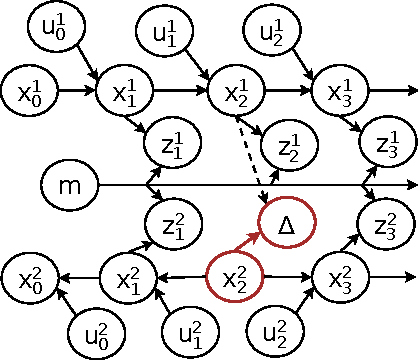
\includegraphics[width=\columnwidth]{{{../FinalFigures/HowardFig3}}}
\caption{Depiction of data integration. Taken from \cite{howard2006multi}.}
\label{fig:HowardFig3}
\end{figure}

While Howard's method is attractive for its speed, it combines the forward and reverse particle weights, which can result in undesired particle error.  In this paper we propose a modification of the algorithm by using independent particle filters for each robot, and demonstrate that the modified algorithm provides a qualitatively better map, and a more accurate pose estimate.

The paper is structured as follows: In \S\ref{S:Back} some background about MRSLAM is provided, the contribution of \cite{howard2006multi} is discussed and a modified scheme is presented.  In \S\ref{S:Alg} the modification of Howard's algorithm \cite{howard2006multi} is discussed.  In \S\ref{S:Exp} the generation of arbitrary data sets, the average time it takes to map 95\% of the environment, and a comparison of Howard's algorithm and the modified algorithm are presented.  \S\ref{S:Conc} rounds out the paper with conclusions and future work.




\section{Background}
\label{S:Back}

\subsection{State of the Art}
\label{SS:Back:SOA}
    
In the literature there are two problems that are often addressed when dealing with MRSLAM:
\begin{enumerate}
\item robot coordination, i.e., how to cover the most area given an unknown environment \cite{julia2012comparison}, and
\item merging the data to create one global map posterior, which is what we will focus on.
\end{enumerate}

In the case where all relative robot poses are known, merging maps is a trivial problem using small modifications to existing SLAM techniques \cite{thrun2001probabilistic}. In the general MRSLAM problem, however, robots may start with unknown absolute and relative poses, and therefore merging of maps requires the discovery of relative relationships between different robot trajectories to build a single map. This is often a costly process, which in general can be solved for robots sharing a search space by estimating each robot's relative pose given a partial map, but this leads to exponential complexity with respect to the number of exploring robots \cite{fox2006distributed}. Nevertheless, several practical algorithms exist to circumvent this naive and inefficient approach,  including coarse topological matching and stitching techniques borrowed from computer vision \cite{birk2006merging}.

In 2006 two schools of thought arouse about how to handle MRSLAM:
\begin{enumerate}
\item Let independent robots build individual maps, then at the end combine the maps together \cite{birk2006merging}.  This approach is particularly attractive for post processing because it requires multiple trial and error to maximize a score function. 
\item On the other hand, there was Howard's paper \cite{howard2006multi}, which uses communication between robots, but requires precisely known relative poses to construct a single global map posterior.
\end{enumerate}
Both had their benefits: \cite{birk2006merging} does not require knowledge of any global or relative poses, but \cite{howard2006multi} can be implemented in real-time.  Because of the real-time nature, and the desire to map as fast as possible, there has also been a great deal of research using \cite{howard2006multi}, but with the added constraint of limited communication \cite{lazaro2013multi}.

In the following subsection we will propose yet another extension to \cite{howard2006multi}.

\subsection{Extension of \cite{howard2006multi}}
\label{SS:Back:Contributions}


Define the weights for a particle filter: $w_t^i$, and the sensor model, $p(z_t|\textbf{x}_t,u_{t-1})$ for the forward and reverse model.  In \cite{howard2006multi}, Howard follows the typical RBPF formulation and defines the un-normalized weight update to be:
\begin{equation}
w^{(i)}_t=p(z_{t}^{f}|\textbf{x}_{t}^{f(i)},m_{t-1}^{(i)}) p(z_{t}^r|\textbf{x}_{t}^{r(i)},m_{t-1}^{(i)}) w^{(i)}_{t-1},
\label{eq:combinedweight}
\end{equation}
where $\bullet^{f(i)}$ and $\bullet^{r(i)}$ denote the forward and reverse elements of particle $(i)$, $\textbf{x}_{t}$ denotes the pose, $z_{t}$ denotes the measurement, and $m_{t-1}$ denotes the map..

In this formulation it is no stretch of the imagination that the forward sensor model and previous weight $p(z_{t}^{f}|\textbf{x}_{t}^{f(i)},m_{t-1}^{(i)}) w^{(i)}_{t-1}$ could be large, denoting a good match to the data in the forward direction, yet the reverse sensor model, $p(z_{t}^{r}|\textbf{x}_{t}^{r(i)},m_{t-1}^{(i)})$, could be small.  Thereby reducing the probability that the best forward direction is resampled.  See for example Fig. \ref{fig:deplete}, particularly particle 1.


Because of this, we propose assuming that the noisy forward and reverse motions are independent, motivates using two particle filters with weights defined by:
\begin{eqnarray}
w^{f(i)}_{t}&=&p(z_{t}^f|\textbf{x}_{t}^{f(i)},m_{t-1}^i)  w^{f(i)}_{t-1}\\
w^{r(i)}_{t}&=&p(z_{t}^r|\textbf{x}_{t}^{r(i)},m_{t-1}^i)  w^{r(i)}_{t-1}
\end{eqnarray}
and with $\{\textbf{x}_{t}^{f(i)},m_{t-1}^i\}$ being resampled using $\{w^{f(i)}_{t}\}$, and $\{\textbf{x}_{t}^{r(i)}\}$ being resampled using $\{w^{r(i)}_{t}\}$.  


\begin{figure}[h]
\centering
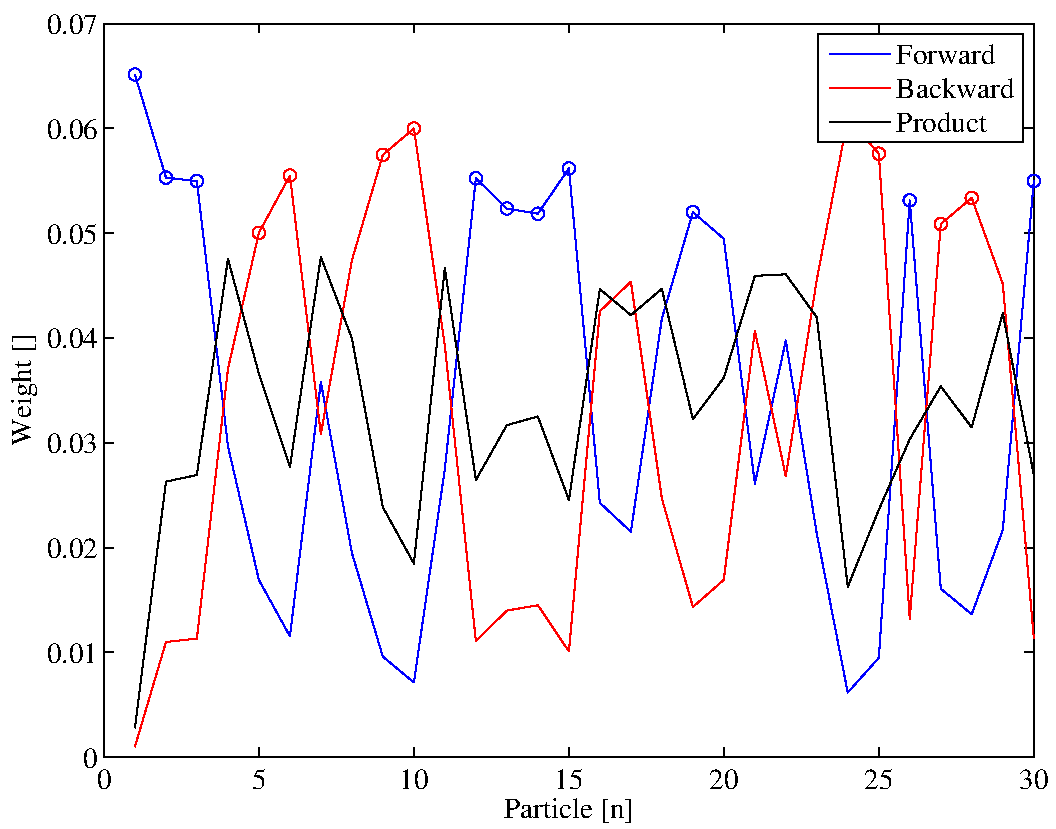
\includegraphics[width=\columnwidth]{../FinalFigures/Depletion}
\caption{Case where the best forward and reverse poses are not chosen. $w^{f(i)}_{t}$ is the forward weight, $w^{r(i)}_{t}$ is the reverse weight, and $w^{(i)}_t$ is the product of the weights.}
\label{fig:deplete}
\end{figure}

Our contribution is two-fold, verifying that Howard's algorithm works, and creating independently sampled particle filters for each mapping robot in the aim to build a more accurate occupancy grid, and obtain a better localization within the map while only marginally increasing the computational complexity.




\section{The Algorithm}
\label{S:Alg}

\subsection{Overview}
\label{SS:Alg:Overview} 


Howard's multi-robot SLAM algorithm generates a single map and pose posterior much in the same way an occupancy grid map SLAM algorithm based on a Rao-Blackwellized particle filter (RBPF) would, but with additions to accommodate multiple robots. Mapping begins with a set consisting of a single robot with known pose and an occupancy grid map of the environment is built as this robot traverses and measures it. The ultimate goal of the algorithm is to simultaneously compute for time $t$, the full SLAM posterior containing all robot pose trajectories $\textbf{x}_{1:t}^i$ and the global map $m_{1:t}$, given only a single known initial pose and sets of measurements
\begin{align*}
p(\textbf{x}_{1:t}^1,\textbf{x}_{1:t}^2&,...,\textbf{x}_{1:t}^M,m_{1:t}|\\&\textbf{x}_0^1,z_{1:t}^1,u_{0:t}^1,\Delta_s^2,z_{1:t}^2,u_{0:t}^2,\Delta_s^3,...,\Delta_s^M,z_{1:t}^M,u_{0:t}^M),
\end{align*}
where $s$ denotes the time of encounter.

The odometry and measurement data of all other robots is stored as it is collected, as it cannot contribute to the global map without a known relative pose linking it to the frame of the first robot. As the first robot encounters additional robots via a mutual pose observation, the newly observed robot is added to the set of mapping robots, and the global map is sequentially conditioned by its actions and measurements. From the point of observation, all future actions and measurements of the new robot are used to condition the map posterior, and likewise all of its previously stored actions and measurements are played back in reverse order from that point as a virtual robot. This information is then passed to a pair of new particle filters for the pose of these robots that contribute to the same global map. Fig. \ref{fig:forwardbackward} gives a graphical example of an encounter where a causal and acausal virtual robot are spawned from a robot encounter.
\begin{figure}[ht]
\centering
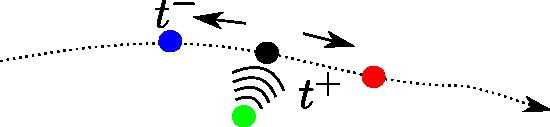
\includegraphics[width=\columnwidth]{../FinalFigures/ForwardBackward.pdf}
\caption{Causal and acausal virtual robots added on encounter.}
\label{fig:forwardbackward}
\end{figure}

As further encounters occur between any robot, real or virtual, in the set of mapping robots and a previously unseen robot, the unseen robot is added to the set of mapping robots and its measured relative pose is again used to establish a reference point with which its actions and measurements can condition the map posterior. Further mutual observations of two robots already in the mapping set are ignored for the sake of simplicity. This encounter-add process is continued recursively for all robots until all stored and future odometry and measurements are exhausted or all possible mapping robots have made an encounter with the mapping set. Beyond this point, the algorithm behaves as a normal RBPF with a stacked state containing pose posteriors of all robots in addition to the map.


This algorithm relies on a number of assumptions that are requisite for it to effectively solve the MRSLAM problem. Firstly, for all explored regions to count towards the map, each mapping robot must have encountered a robot that is an element of the mapping set in order to make a fully connected graph of robot poses, and therefore maximally complete map. Additionally, each robot pose trajectory is independent of all other trajectories such that motion or observation from one robot does not affect another outside of encounter events \cite{howard2006multi}.

\subsection{Algorithm Details}
\label{SS:Alg:Details}
Our implementation of Howard's MRSLAM algorithm follows the basic structure of the below steps that perform data queueing, robot encounter management, and FastSLAM filter updates.
\begin{enumerate}
\item Queue measurement, odometry, and mutual observation (encounter) data.
\item For all robots in the mapping set, take the first element from the queue and update SLAM filter.
\item For all new encounters, split the encountered queue at the present time into causal and acausal queues and instantiate a new set of particles for the causal and acausal trajectory of the observed robot.
\item For all available acausal queues, remove the last element and use it to update the SLAM filter for the corresponding acausal robot.
\item If data includes a prior encounter with a robot not in the mapping set, instantiate a new set of particle for this robot and its acausal virtual self at its location and split the queue for that robot into a causal and acausal queues.
\item Resample all particles to prevent weighting degeneracy.
\item Repeat until all data is consumed.
\end{enumerate}
\vspace{0.1in}
\subsubsection{Data Queueing}
As each robot $R$ collects data, its current odometry $u_t^R$ and measurements $z_t^R$ are added to a running queue data structure before processing. An encounter flag $E_t^R$ and relative pose $\Delta_t^R$, if available, are also added to this queue. 
$$queue_{0:t}^R = append(queue_{0:t-1}^R, \{ u_t^R, z_t^R, E_t^R, \Delta_t^R \})$$
The storing of this data allows for either immediate use by particle filters for robots in the mapping set, or later joining or SLAM filtering after a future encounter with a mapping robot.
\vspace{0.1in}


\subsubsection{Encounters}
An encounter in this sense is defined as the observation of one robot by another mapping robot that produces a relative pose estimate between the robots of $\Delta$. For this implementation, it was assumed that the estimation of $\Delta$ was deterministic for the sake of demonstration and simplicity.

Upon an encounter at time $s$ between Robot $A$ in the mapping set with pose $\textbf{x}_s^A$ and Robot $B$ not in the mapping set with a measured relative pose $\Delta_s^{AB}$, a reference frame pose for each particle $i$ of the newly observed robot is instantiated as the causal particle posterior $\textbf{x}_s^{B(i)}$, and acausal particle pose posterior $\bar{\textbf{x}}_s^{B(i)}$ as:
\begin{eqnarray}
\textbf{x}_s^{B(i)} &= \textbf{x}_s^{A(i)} \oplus \Delta_s^{AB} \\
\bar{\textbf{x}}_s^{B(i)} &= \textbf{x}_s^{A(i)} \oplus \Delta_s^{AB}
\label{eq:relpose}
\end{eqnarray}
Where $\oplus$ is the pose composition operator \cite{smithSelfCheeseman1990}.
At this time, the stored data queue for robot B is also split into a causal queue $queue^B$ and acausal queue $\overline{queue}^B$.
\begin{align*}
\overline{queue}_{t+1:2t}^B = reverse(queue_{0:t-1}^B) \\
queue^B = queue_{t+1:}^B
\end{align*}

If neither robot is within the mapping set and an encounter occurs, this encounter and the associated measured relative pose is stored for later use. In the event that one of these robots later encounters a robot in the mapping set, its virtual acausal robot will spawn another robot pair of the unencountered robot upon backtracking to the location of this initial encounter. At this acausal encounter, the same method of adding relative pose and splitting the queues used in the causal join is used to generate the causal and acausal virtual robots created by this encounter.

Fig. \ref{fig:multiencounter} explains the joining process graphically. The scenario starts with three robots $\textbf{x}_t^1$, $\textbf{x}_t^2$, and $\textbf{x}_t^3$, with $\textbf{x}_t^1$ being the sole robot in the initial mapping set. The actual robots are represented as white circles, the causal particles as red circles (+), the acausal particles as blue circles (-), and encounters as purple arrows. At timestep $T_1$, an encounter occurs between $\textbf{x}_{T_1}^2$ and $\textbf{x}^3$, but neither is in the mapping set at this time, so this encounter is stored. At timestep 2, robots $\textbf{x}_{T_2}^1$ and $\textbf{x}_{T_2}^2$ encounter each other, spawning a causal and acausal pair of pose particles $\textbf{x}^{2+}$ and $\textbf{x}^{2-}$ respectively. $\textbf{x}^{1+}$ and $\textbf{x}^{2+}$ continue propagating forward with new data (not shown) while $\textbf{x}^{2-}$ propagates backwards in time using stored odometry and measurements. The stored encounter between $\textbf{x}_{T_1}^2$ and $\textbf{x}_{T_1}^3$ that was previously stored is then incorporated at time $T_3$ when the acausal particles $\textbf{x}^{2-}$ reach the location of the encounter. This spawns a set of particles for the previously encounter robot $\textbf{x}_{T_1}^3$. As the original encounter happened on the first step, no acausal particles are spawned at this time. As $\textbf{x}^{2-}$ reaches the last remaining pose in the acausal queue, the particles are removed as the past data is exhausted.

%\begin{figure}[ht!]
%\centering
	%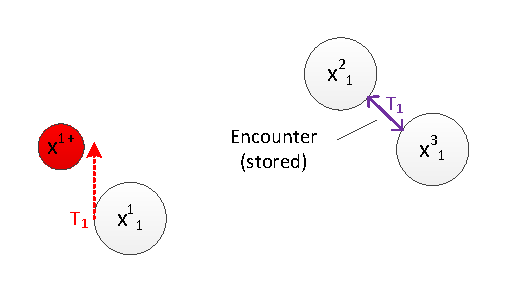
\includegraphics[width=3in]{../FinalFigures/multiencounter_1.pdf} \\
	%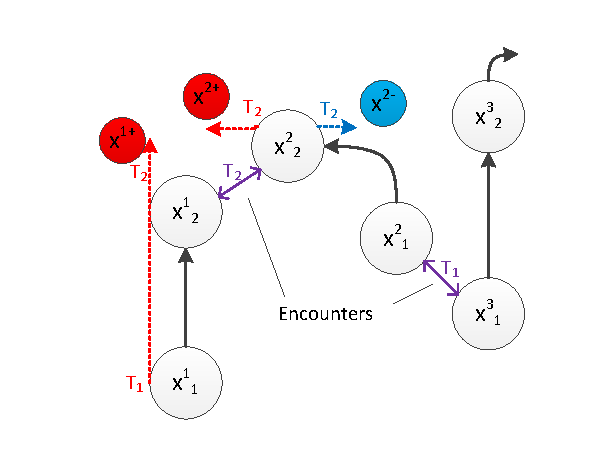
\includegraphics[width=3in]{../FinalFigures/multiencounter_2.pdf} \\
	%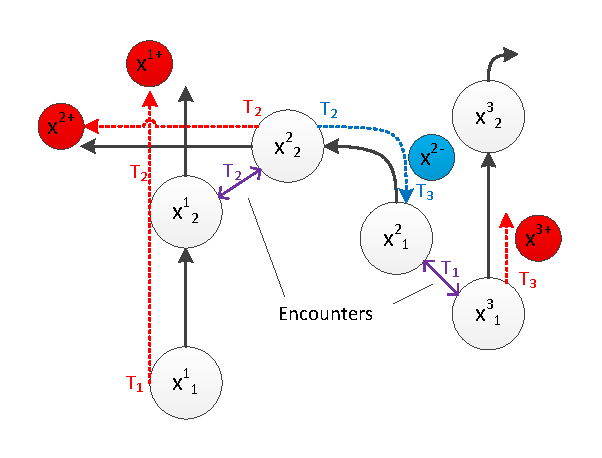
\includegraphics[width=3in]{../FinalFigures/multiencounter_3.pdf} \\
	%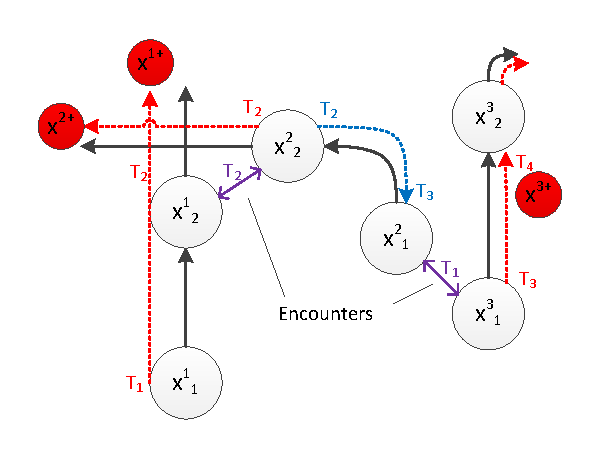
\includegraphics[width=3in]{../FinalFigures/multiencounter_4.pdf} \\
%\caption{Example of Robot Encounters in this MRSLAM Implementation}
%\end{figure}

\newcommand{\codymult}{0.78}
\begin{figure}[ht!]
\centering
    \subfigure[Timestep 1]{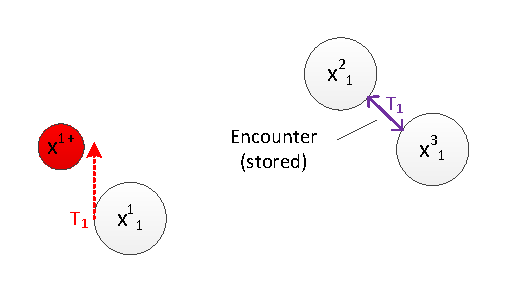
\includegraphics[width=\codymult\columnwidth]{../FinalFigures/multiencounter_1.pdf}} \\
    \subfigure[Timestep 2]{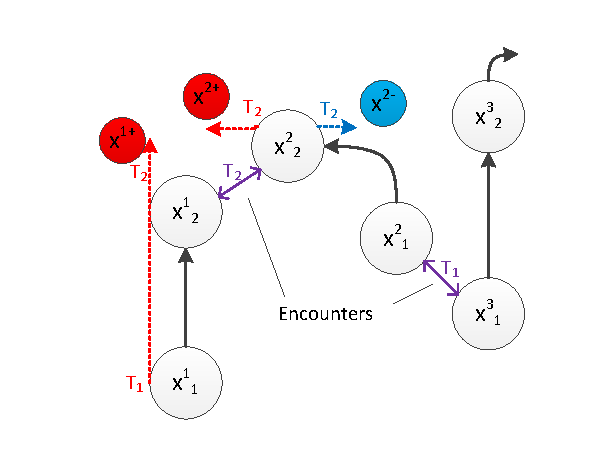
\includegraphics[width=\codymult\columnwidth]{../FinalFigures/multiencounter_2.pdf}} \\
    \subfigure[Timestep 3]{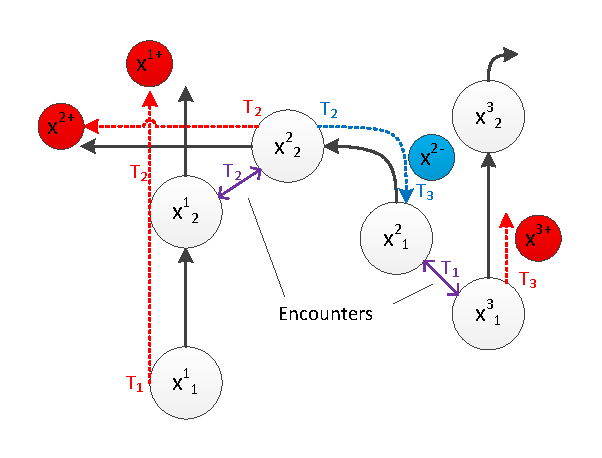
\includegraphics[width=\codymult\columnwidth]{../FinalFigures/multiencounter_3.pdf}} \\
    \subfigure[Timestep 4]{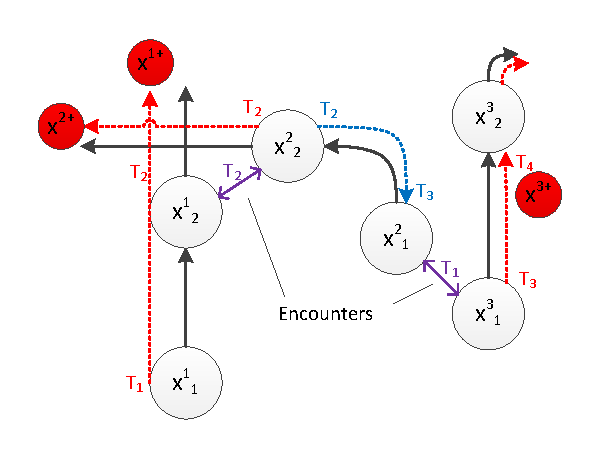
\includegraphics[width=\codymult\columnwidth]{../FinalFigures/multiencounter_4.pdf}} \\
\caption{Example of Robot Encounters in this MRSLAM Implementation}
\label{fig:multiencounter}
\end{figure}

\vspace{0.1in}
\subsubsection{FastSLAM Updates}
At each time-step, the pose posterior is updated for all pose states within the current mapping set and are updated according to a modified Rao-Blackwellized particle filter. Both information from the causal and acausal queues is used to update the SLAM posterior in an almost identical fashion, save for a time-reversed odometry model. 

This process first applies an odometry prediction to each particle. This single update applies to each causal robot particle a forward odometry change given an arbitrary non-linear and noisy forward odometry model $g(x,u)$. For each virtual robot traversing its path in reverse, the next stored point is popped off the corresponding stack and used with a noisy inverse odometry model $\hat{g}_r(x,\bar{u})$
\begin{align*}
\forall \textit{robots $r$} \\
\textbf{x}_{t+1}^{r(i)} &= \hat{g}(\textbf{x}_{t}^{r(i)},u_{t+1}^{r(i)})~~\text{(Causal Prediction)}\\
\bar{\textbf{x}}_{t+1}^{r(i)} &= \hat{g}_r(\bar{\textbf{x}}_t^{r(i)}, \bar{u}_{t+1}^{r(i)}) ~\text{(Acausal Preditiction)}
\end{align*}
Where $\hat{g}$ and $\hat{g}_r$ consist of a deterministic odometry model $g(\textbf{x},u)$ or $g_r(\textbf{x},\bar{u})$ corrupted by model dependent noise $\eta$.
\begin{align}
\hat{g}(\textbf{x},u)&=g(\textbf{x},u)+\eta\\
\hat{g}(\textbf{x},\bar{u})&=g_r(\textbf{x},\bar{u})+\eta
\end{align}

The chosen particle filter implementation allows for a wide choice of assumptions on the distribution of the noise model. Our choice of model used in testing is discussed in the later section on experimental validation.

The odometry prediction step was followed by an occupancy grid map update for each real or virtual robot particle based on current or stored measurements. For each robot $R$, whether it represents causal or acausal particles, the next measurement in the queue, $z_t^R$ is removed and used to update the map for each particle according to a simplified occupancy grid measurement model.

For each particle in $\textbf{x}_t^R$,  the particle's associated map $m_i$, and associated measurement $z_t^R$ is used with the simplified inverse sensor model to compute the log-odds of a particular cell’s occupancy. Our chosen model simulated a typical range, bearing LIDAR type sensor, with a fixed occupied (black) and free (white) probability $p_{occ}$ and $p_{free}$, respectively, and a simple sensor cone model similar to the one shown in Figure \ref{fig:invsensor}. This created the log-odds modifier at time $t$
$$l_{sensor,t,i}=
\begin{cases}
\log\frac{p_{free}}{1-p_{free}} & \text{Cell free}\\ 
\log\frac{p_{occ}}{1-p_{occ}} & \text{Cell Occupied}
\end{cases}$$

\begin{figure}[ht]
\centering
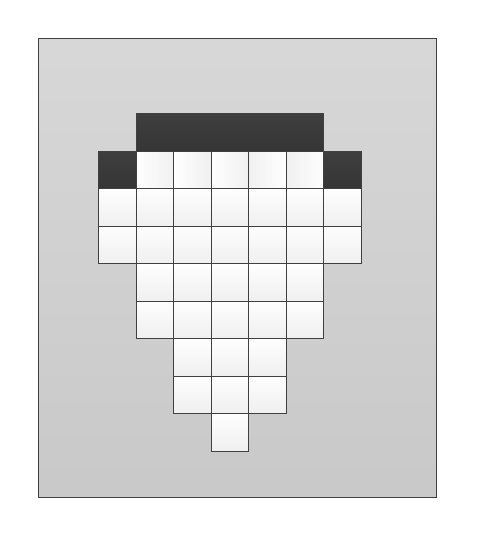
\includegraphics[width=\columnwidth]{../FinalFigures/invsensormodel.pdf}
\caption{Example Inverse Sensor Model Pattern}
\label{fig:invsensor}
\end{figure}

For each cell augmented by the inverse sensor model, the log-odds was updated as:
$$l_{t,i}=l_{t-1,i}+l_{sensor,t,i}-\log\frac{p(m_i)}{1-p(m_i)}$$

All cells uneffected were left at their previous log-odds
$$l_{t,i}=l_{t-1,i}$$

After incorporating the the next measurement for all particles to each map particle, the last portion of the SLAM update consists of updating each pose particle’s weight and resampling to prevent weighting degeneracy.

The weighting of each particle in this step was adjusted using the measurement likelihood given the robot's estimated pose and the current map 
\begin{align}
w^{(i)}=p(z_t^{1(i)}|\textbf{x}_t^{1(i)},m_t)&p(z_t^{2(i)}|\textbf{x}_t^{2(i)},m_t)...\\
&p(z_t^{M(i)}|\textbf{x}_t^{M(i)},m_t)w^{(i)},
\end{align}
where $M$ is the number of robots.

We also implemented an algorithm that assigns an independent particle weighting for each independent pose particle set. For robot R, this weight was computed as:
$$w_t^{R(i)}=p(z_t^{R(i)}|\textbf{x}_t^{R(i)},m_t)w_{t-1}^{R(i)}$$

After the propagation and update, the FastSLAM algorithm performs stochastic universal resampling to generate an update set of uniform weight samples. All weights are normalized such that they sum to 1, a cumulative mass function (CMF) is generated, and a random initial offset is chosen. From this initial offset, an identical number of samples equally spaced across the CMF are taken and the inverse CMF at each of those samples is used to create a new particle. The resulting weights of each particle are then set to a uniform value. 

For our addition where each set of pose particles has independent weights, these weights are used to independently resample each pose set while leaving the map unchanged. Stochastic universal resampling is also used for this process.
\vspace{0.1in}
\subsubsection{Commentary on Sequential Updating}
By only incorporating a fixed number of odometry and measurement updates in a given timestep, Howard's MRSLAM algorithm places a bound on computation time \cite{howard2006multi}. Each particle propagation, and map update, and measurement model weighting computation are constant time operations for a fixed map size. This results in bounds on computational complexity for a fixed map size using $M$ robots each with $n$ particles of $\mathcal{O}(mn)$. Incorporating all past measurements simultaneously would require computing a possibly large number of particle filter updates \cite{howard2006multi}. Using Howard's algorithm, where particle weights are shared across all poses, would also be at risk of resampling impoverishment where existing particles would die out as a result of a simultaneous incorporation of all acausal data at an encounter.



\section{Experimental Validation}
\label{S:Exp}

In this section we present how the data set was generated, the time it takes to map 95\% of the environment, and a comparison between using Howard's algorithm and the independently sampled algorithm.  




\subsection{The Data Set}
\label{S:Exp:DataSet}

The data set consists of PAS triple $(\textbf{x}^{R(i)}_t,u^{R(i)}_t,z^{R(i)}_t)$, where $R$ denotes the robot ID, and $t$ denotes the time.  The pose, $\textbf{x}^{(i)}_t$, is comprised of the $x_t^R$-$y^R_t$ position, as well as the orientation $\theta^R_t$.  The input, $u^R_t$, is composed of the position deflection, $\delta^R_t$, and the angular deflection, $\omega_t$.  Finally, the measurements, $z^R_t$, contains scan data for rays cast out at $1^\circ$ intervals from $[-90^\circ,90^\circ]$, to simulate a laser scan.  

To obtain the measurements a binary map, $I$, and the ray-circle intersection algorithm.

\subsubsection{Ray-Circle Intersection}

The scan data is constructed using ray-circle intersection of a binary image, $I$ (like that of Fig. \ref{subfig:Enc} without the paths).  The idea of ray-circle intersection is to find all the object pixels within a region of interest (ROI), in this case the shaded pixels in the semi-circle, $I_{semi}$, as seen in Fig. \ref{subfig:raycirc}, 
\begin{equation}
I_{semi}=\left\{I_{xy}\in I |\  ||I_{xy}-I_{\textbf{x}_t^R}||_2^2<r^2 \right\},
\label{eq:Isemi}
\end{equation}
where $I_{\textbf{x}_t^R}$ is the position of the robot $R$ in the map, and $I_{xy}$ denotes the pixels $(x,y)$.

Then $I_{semi}$ is intersected with the object, $I_{obj}=\{I_{xy}\in I | \ I_{xy}=1\}$ (the filled squares in Fig. \ref{subfig:raycirc}, to get $I_{filled}$.  A ray is then defined by 
\begin{equation}
\textbf{v}_k=\begin{bmatrix}
I_{x_t^R}+r_k^j \cos(\phi_k)\\
I_{y_t^R}+r_k^j \sin(\phi_k)\\
\end{bmatrix}, 
\label{eq:ray}
\end{equation}
where $r_k^j>0$ is some partitioning of the length of the ray up to the maximum range of the sensor.  This ray is intersected with $I_{filled}$ to get $I_{ray}$ (colored in orange in Fig. \ref{subfig:raycirc}).  Finally, the minimum distance to the object, $r_{k}^*$ , is selected (the $r_k^j$ corresponding the blue square in Fig. \ref{subfig:rstar}) to get the distance measurement $z_t^{R,k}$ of the object to the robot.  

\begin{equation}
r_k^*=\min_{j} r_{k}^j
\end{equation}


\begin{figure}[ht]
\centering
\subfigure[$I_{filled}$ and the intersection with the ray $\textbf{v}_k$.]{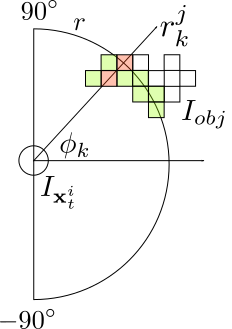
\includegraphics[height=4cm]{../FinalFigures/RayCircleIntersection1}\label{subfig:raycirc}}
\subfigure[The selection of $r_k^*$.]{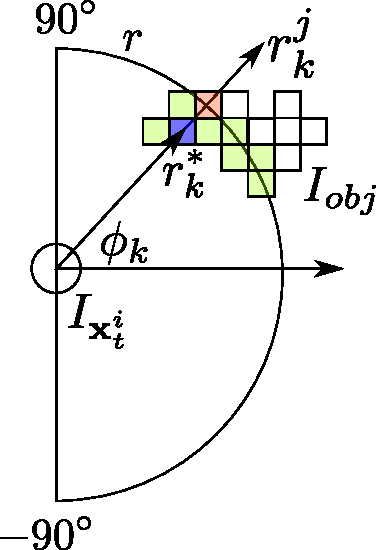
\includegraphics[height=4cm]{../FinalFigures/RayCircleIntersection}\label{subfig:rstar}}
\caption{Visualization of ray-circle intersection algorithm.}
\label{fig:raycirc}
\end{figure}

To obtain experimental-like data, we introduce zero mean, additive Gaussian noise with variance $Q$ to $z_t^{R,k}$ to get noisy measurements $\hat{z}_t^{R,k}$:
\begin{equation}
\hat{z}_t^{R,k}=z_t^{R,k}+\mathcal{N}(0,Q).
\end{equation}

\subsubsection{Wall Following}

For our coordination, we use wall following to search the environment.  The specifics of this implementation are: wall following is turned on when $t\in[50,200]$, each robot is equipped with a parity bit to ensure that some robots move in opposite directions, and if the robot happens to get stuck in a loop, wall following will temporarily turn off.

Using wall following to search the environment led to the choice of the odometry motion model, because wall following can be easily implemented in conjunction with scan data obtained using ray-circle intersection.


\subsubsection{The Odometry Motion Model}

The motion model used was a classic odometry motion model.  
\begin{equation}
\begin{bmatrix}
x_{t}\\
y_{t}\\
\theta_{t}
\end{bmatrix}=\begin{bmatrix}
x_{t-1}\\
y_{t-1}\\
\theta_{t-1}
\end{bmatrix}+\begin{bmatrix}
\hat{\delta}_{t-1}  \cos(\theta_t+\hat{\omega}_t)\\
\hat{\delta}_{t-1}\sin(\theta_t+\hat{\omega}_t)\\
\hat{\omega}_{t-1}
\end{bmatrix},
\label{eq:OdometryMotion}
\end{equation}
where
\begin{eqnarray}
\hat{\delta}_{t-1}&=&\delta_{t-1}-\mathcal{N}(0,\alpha_1\delta_{t-1}^2+\alpha_2\omega_{t-1}^2)\\
\hat{\omega}_{t-1}&=&\omega_{t-1}-\mathcal{N}(0,\alpha_3\delta_{t-1}^2+\alpha_4\omega_{t-1}^2).
\end{eqnarray}

This results in the reverse odometry model:
\begin{equation}
\begin{bmatrix}
x_{t-1}\\
y_{t-1}\\
\theta_{t-1}
\end{bmatrix}=\begin{bmatrix}
x_{t}\\
y_{t}\\
\theta_{t}
\end{bmatrix}-\begin{bmatrix}
\hat{\delta}_t  \cos(\theta_t-\hat{\omega}_{t-1})\\
\hat{\delta}_{t}\sin(\theta_t-\hat{\omega}_{t-1})\\
\hat{\omega}_{t-1}
\end{bmatrix}.
\label{eq:ReverseOdometryMotion}
\end{equation}

With these motion models we may now discuss how the robot encounters and determines relative poses.  


\subsubsection{Encounter Detection and Relative Pose}

In place of using a hypothetical camera to determine if robot encounters occur, we use the ray-circle intersection algorithm.  We treat each robot as an object in the binary image, $I$, and if a $(r_k^*,\phi_k)$ is found to coincide with an added robot, and encounter is declared and a relative pose is calculated is calculated from \eqref{eq:relpose}.



\subsubsection{The Environment, Robot Trajectories, and Encounters}

  Fig. \ref{subfig:Encvst} shows at what time a robot encountered another, note: only the first encounter is used.

Fig. \ref{subfig:Enc} shows the binary map of the environment, the paths each robot took (solid lines), the point when a robot encounter occurred (dashed gray lines), where the first encounter occurred (thick grey line), the particles at the final time step (attached to the solid lines), and the global pose (corresponding circles) for comparison.

For ease of use, we will set Robot 1's initial pose as the global frame's origin.  

\begin{figure}[ht]
\centering
\subfigure[Robot encounters versus time.]{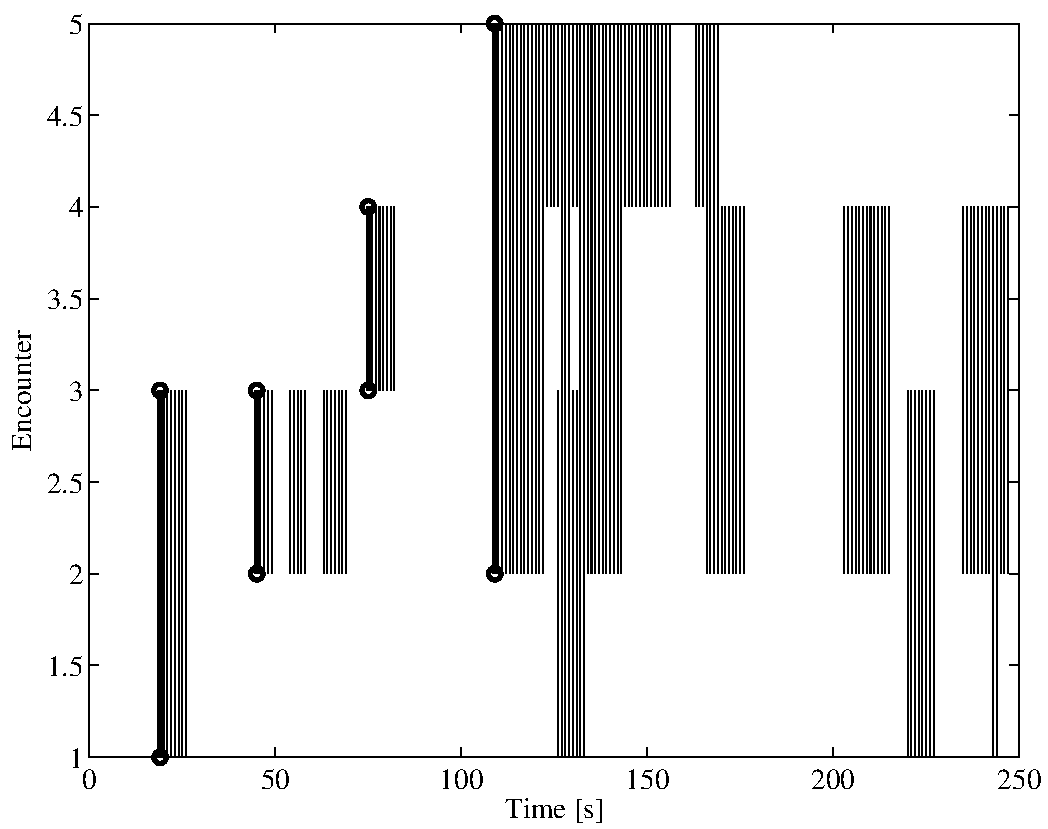
\includegraphics[width=\columnwidth]{../FinalFigures/EncountersTimes}\label{subfig:Encvst}}
\subfigure[The test geometry, robot paths (colored lines), and encounters (dashed gray lines).]{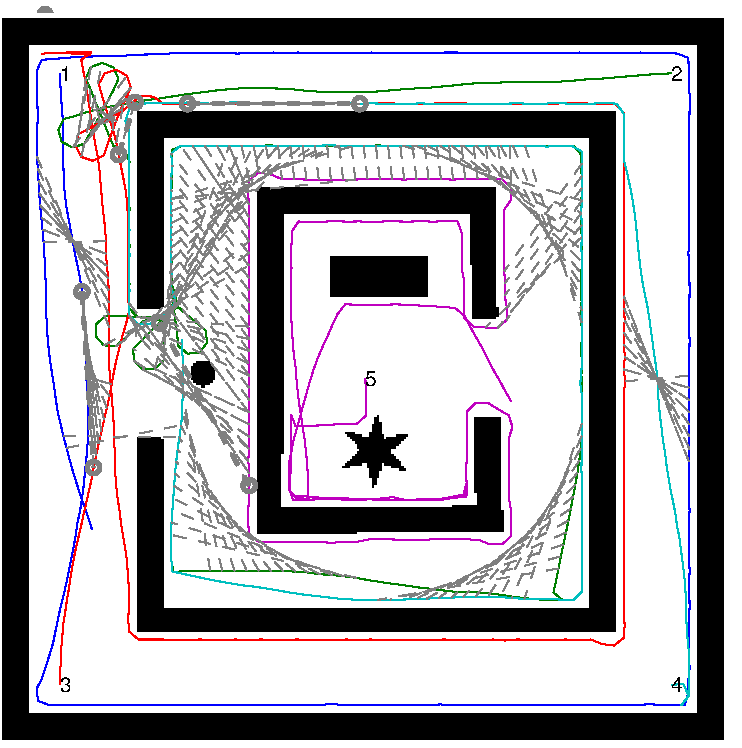
\includegraphics[width=\columnwidth]{../FinalFigures/Encounters}\label{subfig:Enc}}
\caption{Environment geometry, robot paths, and encounters.}
\label{fig:EnvEnc}
\end{figure}



\subsection{Timing}
\label{S:Exp:Timing}

One of the primary motivations for using MRSLAM is to decrease the amount of time it takes to complete the mapping objective.  In this section we demonstrate that generally speaking the time it takes to map an environment decreases with the number of robots.  

To present the time it takes to map the environment, we must first define what we mean by mapping the environment.  When we say that we have mapped an environment, we mean that we have created an occupancy grid, $J$, that matches the outermost black edges of Fig. \ref{subfig:knownpose} using a perfect sensor/actuator.  

To obtain the edges of the binary map, $I$, we use morphological erosion to obtain $\tilde{I}$:
\begin{equation}
\tilde{I}=I\ominus \begin{bmatrix}
1 & 1 & 1 \\
1 & 1 & 1 \\
1 & 1 & 1
\end{bmatrix},
\end{equation}
then padding $\tilde{I}$ with zeroes, we take the exclusive or of $I$ and $\tilde{I}$ to $I_{edge}$:
\begin{equation}
I_{edge}=(\tilde{I}\wedge \neg I)\vee (\neg \tilde{I}\wedge I).
\end{equation}
Then we define the percent mapped as
\begin{equation}
\zeta =\frac{\sum_{x,y}I_{edge}\wedge J}{\sum_{x,y}I_{edge}},
\end{equation}
and when $\zeta\geq 0.95$, we say that the environment has been mapped.

Using 100 different trials, Table \ref{table:timing} provides the average amount of time it took to map 95\% of the environment using different number of robots.  To note is that the averages do tend to decrease as expected.  However, it should be noted that there is a large degree of uncertainty, at least until we get beyond 7 robots.  

\begin{table}
\centering
\caption{Time to map 95\% of the environment.}
\label{table:timing}
\begin{tabular}{c|c|c|c|c}
\hline
\hline
\# Robots & Mean & Std  & Max & Min \\
\hline
1 &  501.5185  &  99.4  & 684  & 341\\
\hline
2 &  357.3182  & 170.8  & 654  & 162\\
\hline
3 & 201.8646   & 92.4  & 549  & 122\\
\hline
4 &  332  & 179.2 & 681  & 140\\
\hline
5 &  212.8191  & 113.4  & 523  & 117\\
\hline
6  & 242.4524  & 120.7  & 594  & 100\\
\hline
7  & 262.9425  & 134.3  & 681  &  79\\
\hline
8  &  74.1717  &  20.1 &  150  & 55\\
\hline
9  &  72.0101  &  27.4  & 257   & 54\\
\hline
10  &  56.9600  &   6.3  &  91  &  48\\
\hline
\hline
\end{tabular}
\end{table}



\subsection{The Results}
\label{S:Exp:Results}

\newcommand{\multiplier}{7.25cm}
\begin{figure*}[th]
\centering
\subfigure[Pure Odometry, high noise.]{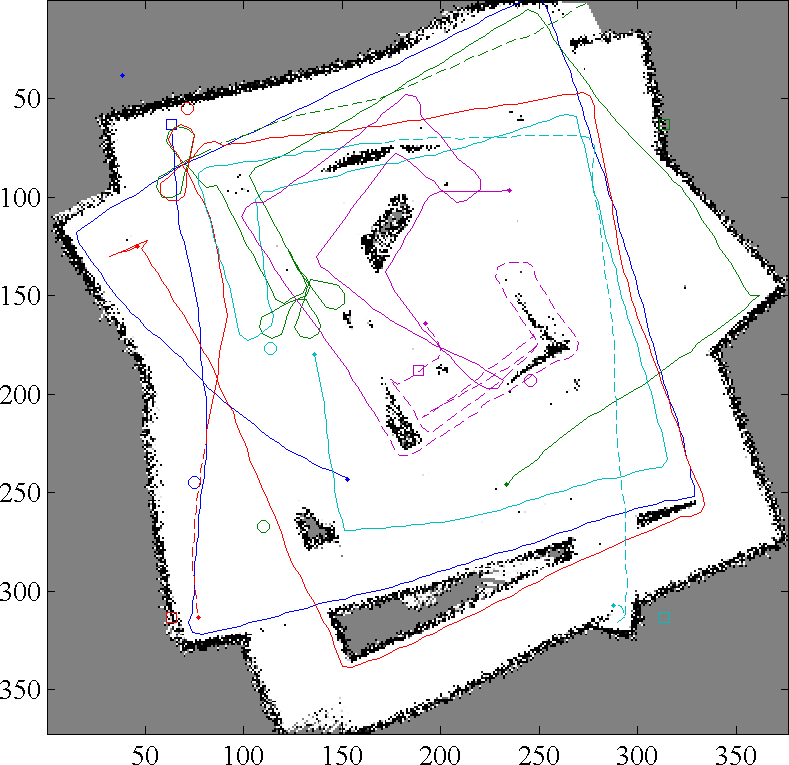
\includegraphics[width=\multiplier]{../FinalFigures/PureOdometry}\label{subfig:pureodom}}
\subfigure[Known Poses]{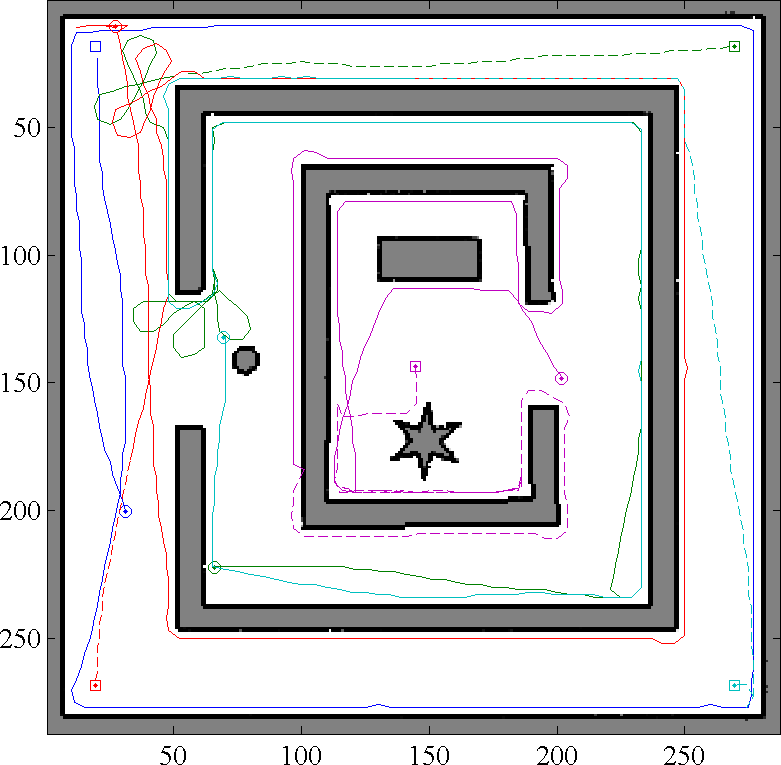
\includegraphics[width=\multiplier]{../FinalFigures/KnownPoses}\label{subfig:knownpose}}\\
\subfigure[Howard Implementation: Unknown Poses, low noise.]{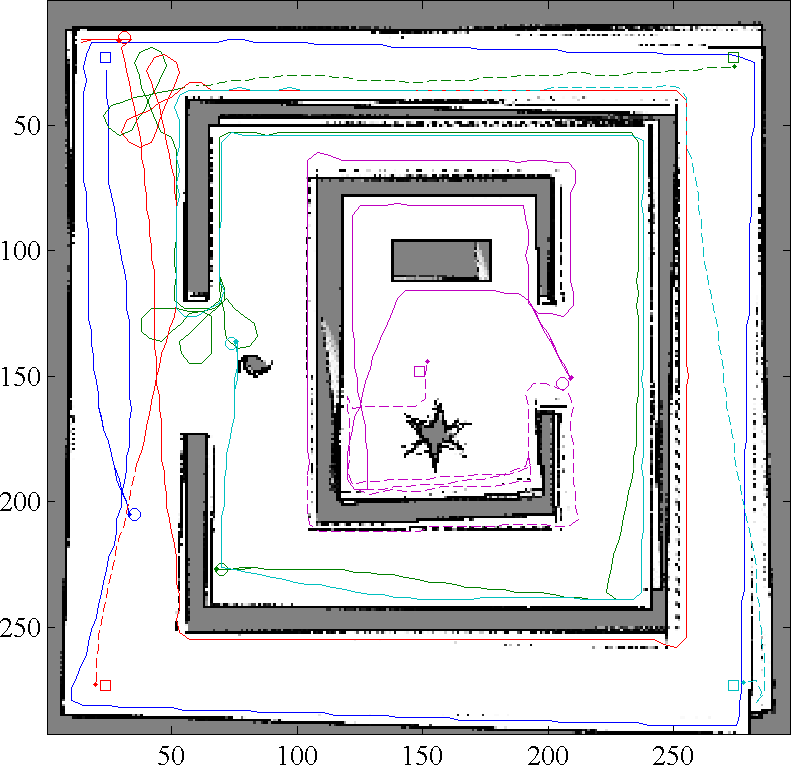
\includegraphics[width=\multiplier]{../FinalFigures/HowardLowNoise}\label{subfig:HowardLow}}
\subfigure[Proposed Implementation: Unknown Poses, low noise.]{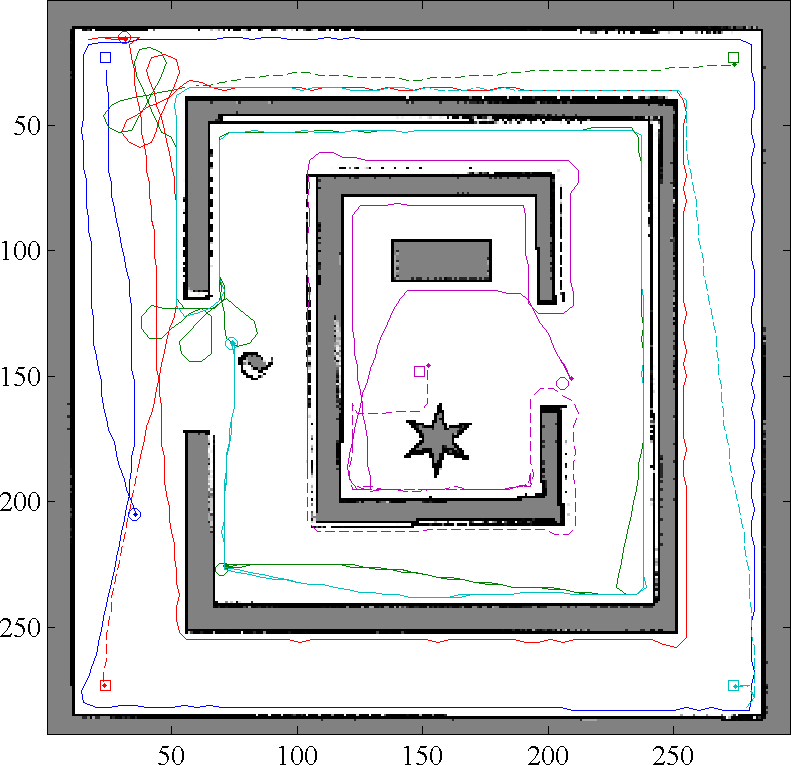
\includegraphics[width=\multiplier]{../FinalFigures/OursLowNoise}\label{subfig:OurLow}}\\
\subfigure[Howard Implementation: Unknown Poses, High noise.]{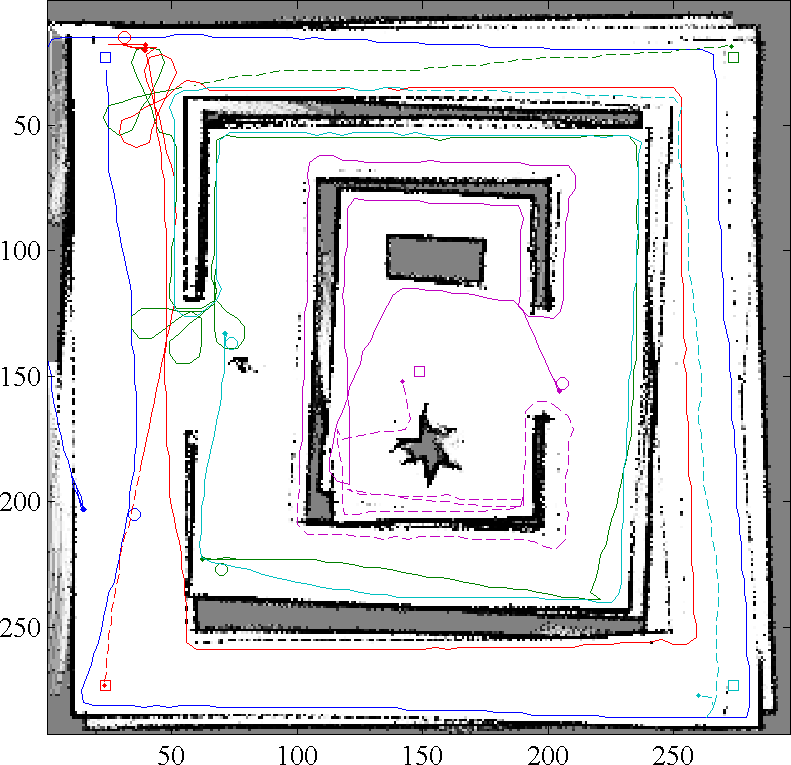
\includegraphics[width=\multiplier]{../FinalFigures/HowardHighNoise}\label{subfig:HowardHigh}}
\subfigure[Proposed Implementation: Unknown Poses, High noise.]{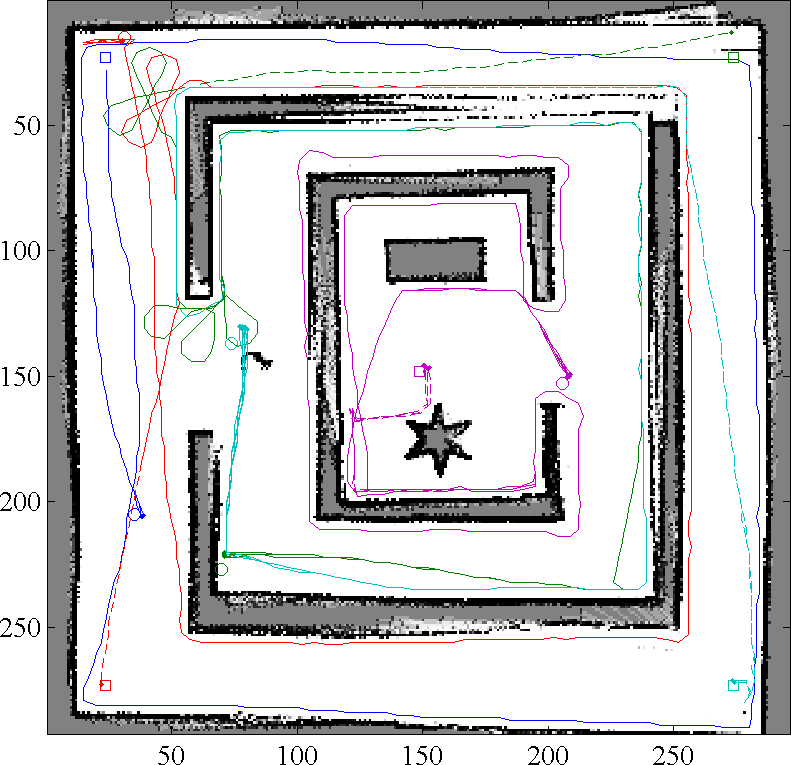
\includegraphics[width=\multiplier]{../FinalFigures/OursHighNoise}\label{subfig:OurHigh}}
\caption{Comparison between Howard's implementation and the proposed implementation.}
\label{fig:Comp}
\end{figure*}

From Table \ref{table:timing} we see that there is a large drop-off when we increase the number of robots from 2$\rightarrow$3, 4$\rightarrow$5, and 7$\rightarrow$8.  Despite it has the highest average time, 5 robots nicely conveys the complexity that can be achieved; as such, 5 robots, each with 30 particles, will be used to highlight the improvement of the independently sampled algorithm over Howard's using a 250 second simulation.  

To compare the two algorithms, we use two sets of sensor/actuator data: a low noise set and a high noise set. 
\begin{description}
\item[\textbf{Low}] The low noise set perturbs the actuator input by $\mathcal{N}(0,0.1)\ [m]$ on $\delta_t^{R}$, $\mathcal{N}(0,0.01)\ [m]$ on $\omega_t^{R}$, and $\mathcal{N}(0,0.5)\ [m]$ on $z_t^{R,k}$.  
\item[\textbf{High}] The high noise set perturbs the actuator input by $\mathcal{N}(0,1)\ [m]$ on $\delta_t^{R}$, $\mathcal{N}(0,0.1)\ [m]$ on $\omega_t^{R}$, and $\mathcal{N}(0,1.5)\ [m]$ on $z_t^{R,k}$.
\end{description}

The qualitative results are presented in Fig. \ref{fig:Comp}.  Fig. \ref{subfig:pureodom} provides the occupancy grid if pure odometry was used, to contrast the poor performance the occupancy grid using known poses is given in Fig. \ref{subfig:knownpose}.

For Fig. \ref{subfig:HowardLow} and \ref{subfig:HowardHigh}, the solid and dashed line represent the best estimated trajectory in the causal and acausal directions.  Whereas, for Fig. \ref{subfig:OurLow} and \ref{subfig:OurHigh}, the solid and dashed lines represent the best estimated path for the causal and acausal data, respectively.

Fig. \ref{subfig:HowardLow}-\ref{subfig:OurHigh} provide the comparison between Howard's and the proposed algorithm.  Comparing Fig. \ref{subfig:HowardLow} and \ref{subfig:OurLow}, it is easy to see that the proposed implementation is almost as good as the occupancy grid with known poses (Fig. \ref{subfig:knownpose}).  Even in the high noise case, Fig. \ref{subfig:HowardHigh} and \ref{subfig:OurHigh}, we see less error with the independently sampled algorithm.  

Over the number of particles, we define the minimum sum of squares error (a.k.a. the least absolute deviation error):
\begin{equation}
\varepsilon=\min_{k\in\{1,\cdots,n\}}\sqrt{\sum_{R=1}^{M} ||\textbf{x}_{t}^R-\hat{\textbf{x}}^{R,k}_{t}||^2_2}
\end{equation}
where $n$ is the number of particles, $M$ is the number of robots, and $\textbf{x}_t^R$ is the known pose, $\hat{\textbf{x}}^{R,k}_{t}$ is pose of particle $k$ in the global frame.  Using this measure, Fig. \ref{fig:minsumerr} quantitatively demonstrates that the independently sampled algorithm provides a better estimate of the pose for nearly all time instants.  Note: for the first 100 seconds, both techniques have the same error, but for the high noise case, the independently sampled algorithm dominates with less than half the error of Howard's algorithm.  Enclosed are videos highlighting Fig. \ref{fig:Comp}.




\begin{figure}[h]
\centering
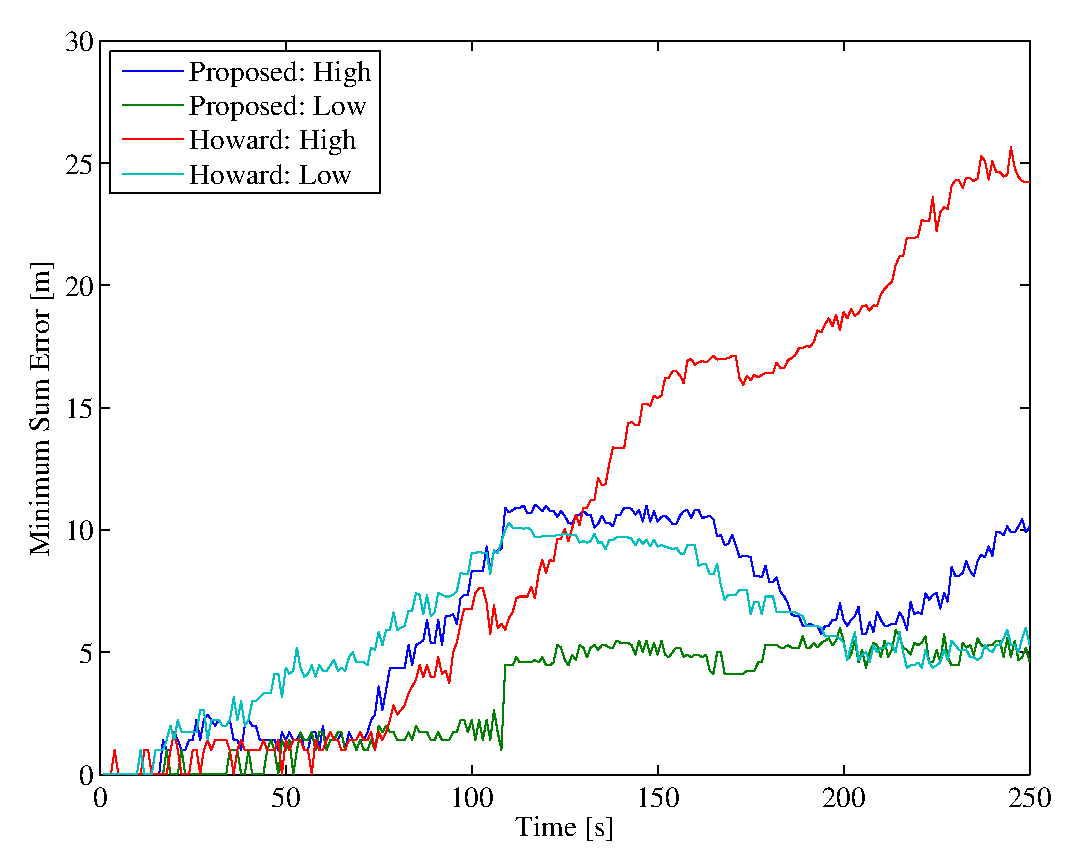
\includegraphics[width=\columnwidth]{../FinalFigures/MinSumError}
\caption{Minimum sum square error versus time.}
\label{fig:minsumerr}
\end{figure}

\begin{frame}
\frametitle{Conclusions}
\begin{itemize}
\item Conclusions:
\begin{itemize}
\item 
\end{itemize}
\item Future work:
\begin{itemize}
\item Decrease 
\item Make it work on Albert B data set
\end{itemize}
\end{itemize}
\end{frame}

\bibliographystyle{plain}
\bibliography{Citations}

%%%%%%%%%%%%%%%%%%%%%%%%%%%%%%%%%%%%%%%%%%%%%%%%%%%%%%%%%%%%%%%%%%%%%%%%%%%%%%%%
\addtolength{\textheight}{-12cm}   % This command serves to balance the column lengths
                                  % on the last page of the document manually. It shortens
                                  % the textheight of the last page by a suitable amount.
                                  % This command does not take effect until the next page
                                  % so it should come on the page before the last. Make
                                  % sure that you do not shorten the textheight too much.

%%%%%%%%%%%%%%%%%%%%%%%%%%%%%%%%%%%%%%%%%%%%%%%%%%%%%%%%%%%%%%%%%%%%%%%%%%%%%%%%



%%%%%%%%%%%%%%%%%%%%%%%%%%%%%%%%%%%%%%%%%%%%%%%%%%%%%%%%%%%%%%%%%%%%%%%%%%%%%%%%



%%%%%%%%%%%%%%%%%%%%%%%%%%%%%%%%%%%%%%%%%%%%%%%%%%%%%%%%%%%%%%%%%%%%%%%%%%%%%%%%





\end{document}
